\begin{figure}[h!]
	 \centering 
	 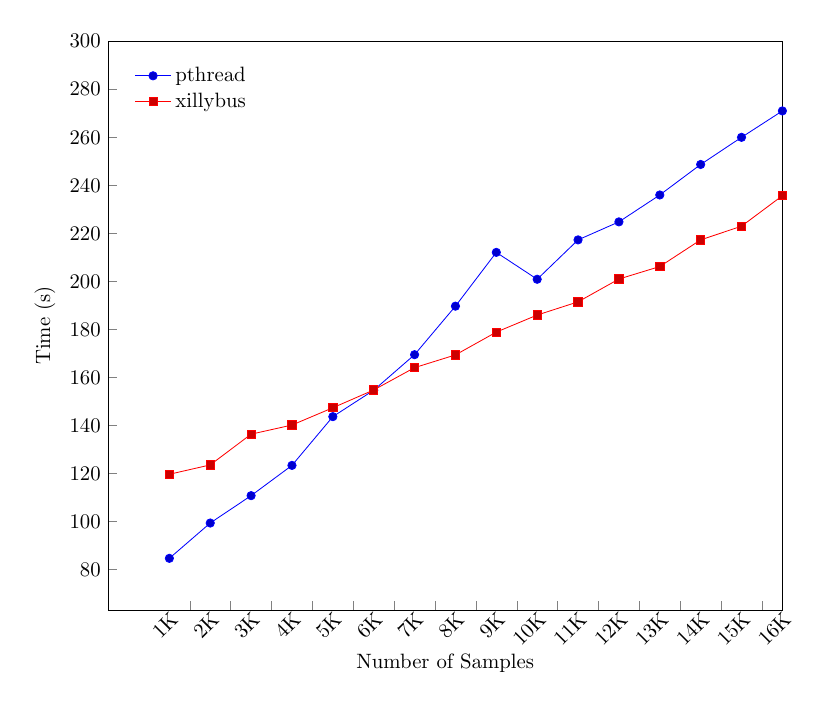
\begin{tikzpicture}[scale = 0.75]
	 \begin{axis}[
    	xlabel=Number of Samples,
		ylabel=Time ($\upmu$s),
	 	xtick pos=left,
		ytick pos=left,
		ymax = 300,
		xmax = 16384,
   		symbolic x coords={1024, 2048, 3072, 4096, 5120, 6144, 7168, 8192, 9216, 10240, 11264, 12288, 13312, 14336, 15360, 16384},
	 	xtick=data,
		xticklabels={1K, 2K, 3K, 4K, 5K, 6K, 7K, 8K, 9K, 10K, 11K, 12K, 13K, 14K, 15K, 16K},
	 	width = 13cm,
	 	xmode = normal,
	 	legend pos=north west,
	    legend style={draw=none},
	 	x tick label style={rotate=45, anchor=north east, inner sep=0mm},
		major x tick style = {opacity=0},
		minor x tick num = 1,
		minor tick length=1ex,
		every node near coord/.append style={
        anchor=west,
        rotate=90,
        font=\tiny
		},
	 ]    
   
	\addplot plot coordinates {
	    (1024,     84.7)
		(2048,     99.4)
		(3072,    110.8)
		(4096,    123.4)
		(5120,    143.7)
		(6144,    154.7)
		(7168,   169.5)
		(8192,   189.7)
		(9216,     212.1)
		(10240,     200.9)
		(11264,    217.3)
		(12288,    224.8)
		(13312,    236)
		(14336,    248.7)
		(15360,   260)
		(16384,   271)
		};

	\addplot plot coordinates {
	    (1024,     119.7)
		(2048,     123.6)
		(3072,    136.4)
		(4096,    140.2)
		(5120,    147.4)
		(6144,    154.8)
		(7168,   164.1)
		(8192,   169.4)
		(9216,     178.9)
		(10240,    186)
		(11264,    191.5)
		(12288,    201)
		(13312,    206.2)
		(14336,    217.3)
		(15360,   223)
		(16384,   235.7)
		};
 
    \legend{pthread\\xillybus\\} 
	\end{axis}
	\end{tikzpicture} 
	\label{writebuffer} 
	\caption{Timing Analysis for clEnqueueWriteBuffer API} 
	\label{graph1:write}
\end{figure}